\chapter{Архитектура искусственных нейронных сетей}

\section{Общая теория нейронных сетей}
Искусственная нейронная сеть (ИНС)~--- математическая модель, 
которая работает по принципу, аналогичному работе сетей нервных клеток живого организма.
ИНС основана на наборе связанных между собой узлов, 
называемых искусственными нейронами, которые моделируют биологические нейроны~--- клетки,
которые принимают на вход информацию (сигналы) от~других нейронов, обрабатывают~ее, а~затем передают 
другим нейронам посредством электрических сигналов.

В математической модели нейрона ядро, где накапливается заряд, заменяется на \textit{сумматор}. 
Дендриты, по которым сигнал приходит от других нейронов в ядро нейрона, заменяются на~\textit{входы} в сумматор.
Сила синапсов моделируется при помощи \textit{весов}, которые задаются для~каждого из~входов.
Аксон, по~которому нейрон отправляет сигналы к другим нейронам, соответствует \textit{выходу} сумматора.
Далее сигнал проходит через \textit{функцию активации}, после чего уходит 
к другим нейронам. Простейшая функция активации~--- пороговая:
\begin{equation*}\label{key}
f(z) = \begin{cases}
1,~z>0,\\
0,~z\leq 0.
\end{cases}
\end{equation*}

Иными словами, для~$ n $ входов сумматора $ \vec{x} = (x_1, x_2,\ldots, x_n) $ с~заданными весами $ \vec{w} = (w_1, w_2,\ldots, w_n) $ и~смещением~$ b $, выходной сигнал есть
\begin{equation*}
y = f(z) = f(w_1 x_1 + w_2 x_2 + \ldots + w_n x_n + b) = f(\vec{x}\cdot\vec{w} + b),
\end{equation*}
где $f$~--- функция активации нейрона.

Таким образом, нейрон как объект производит некоторую \textit{линейную} операцию, которая задаётся двумя параметрами: 
вектор весов и смещение. Эти параметры настраиваются в~процессе обучения ИНС.

Разделяющая поверхность в~соответствующем гиперпространстве
задаётся уравнением $$ \vec{x}\cdot\vec{w} + b = 0, $$ 
определяющим гиперплоскость в пространстве весов $ \vec{w}\in\mathcal{R}^n $, причем вектор 
$ \vec{w} $ является нормалью к этой гиперплоскости. Получается, что один 
нейрон даёт \textit{линейную} разделяющую поверхность. 
Если же соединить нейроны в~некоторую более сложную конструкцию (то~есть ИНС), 
возможно получить \textit{нелинейные} разделяющие поверхности.


\section[Полносвязные нейронные сети прямого\\ распространения]{Полносвязные нейронные сети\\ прямого распространения}

Полносвязная нейронная сеть прямого распространения (англ. feed forward neural networks, FFNN)~--- сеть, 
которая представляет из себя
набор слоев, где каждый слой состоит из~входных, скрытых или выходных нейронов. 
В~простейшем случае это выглядит следующим образом:
\begin{figure}[!h]
	\centering
	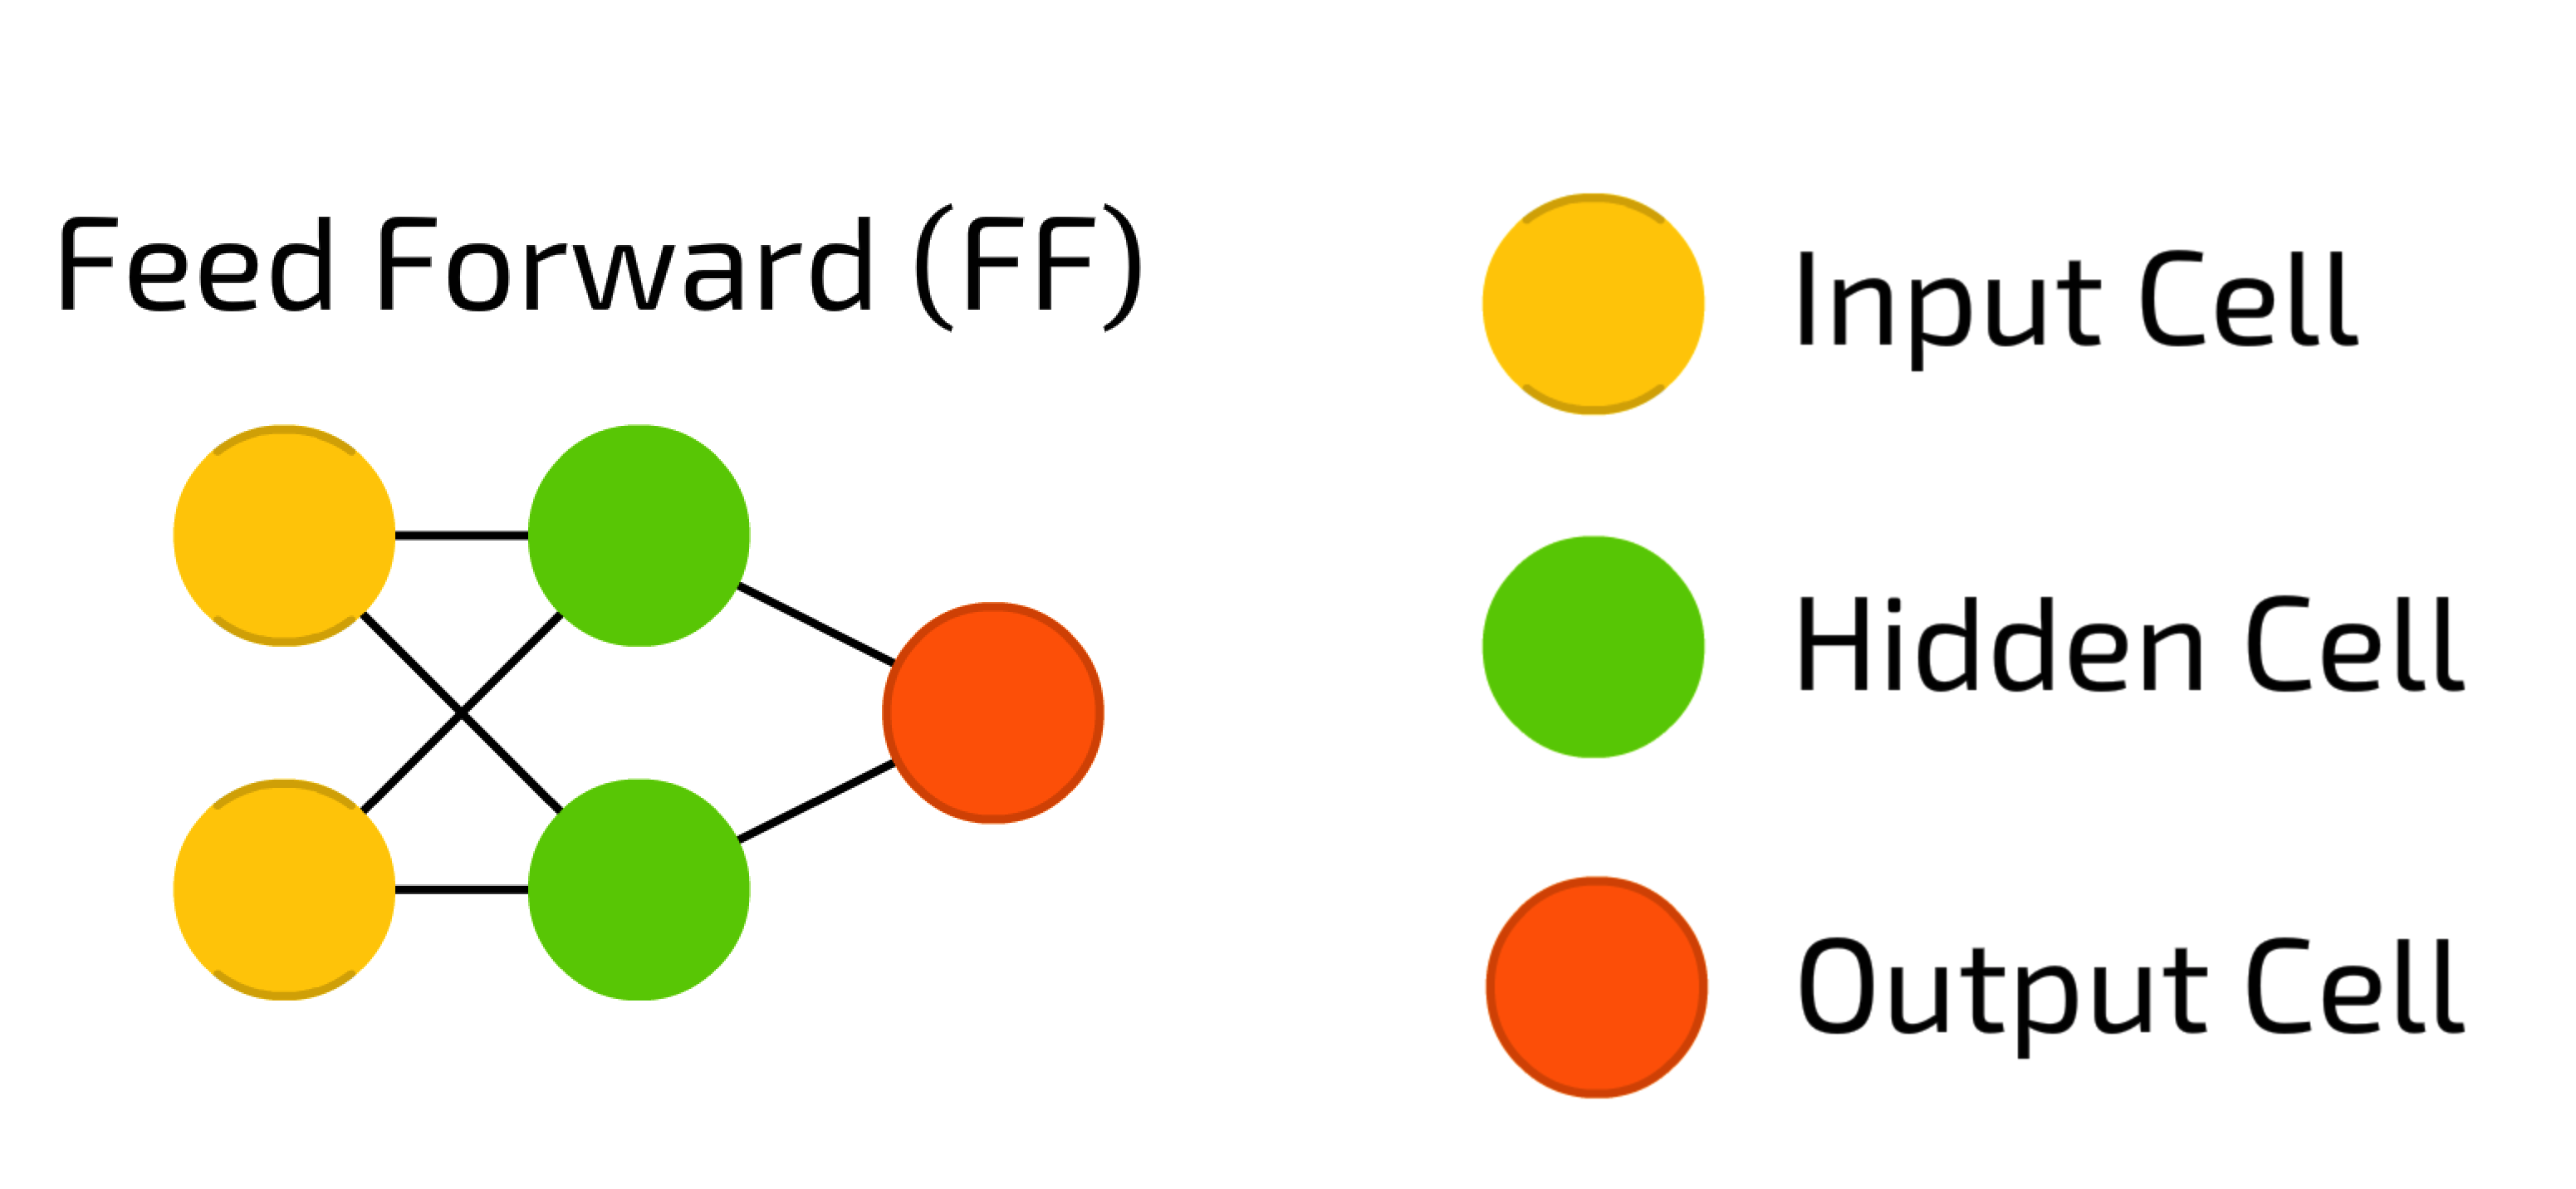
\includegraphics[width=0.7\textwidth]{pics/FFNN}
	\caption{Полносвязная НС}
	\label{FFNN}
	% МЫЫЫЛО %почему мыло, у меня вроде все ок
\end{figure}

Нейроны одного слоя не связаны между собой, в~то~время как соседние слои \textit{полносвязны} (англ. fully connected, FC), т.\,е. каждый нейрон связан со всеми 
нейронами предыдущего слоя, причем все связи направлены строго от входных нейронов к~выходным. 

Данный тип сетей обычно обучается по методу обратного распространения ошибки (англ. backpropagation, BP) \cite{backprop}, 
в котором сеть получает множества входных и выходных данных. Эта ошибка 
зависит от выбранной \textit{функции потерь} (loss function), которая определяет величину 
ошибки между входом и выходом. 

Этот процесс называется обучением с учителем.
От~обучения без~учителя он~отличается тем, что в~последнем случае 
множество выходных данных сеть составляет самостоятельно.
Если сеть имеет достаточное количество 
скрытых нейронов, она теоретически способна смоделировать взаимодействие между 
входными и выходными данными.

Однако данный тип сетей имеет следующие существенные недостатки:
\begin{enumerate}
	\item \textbf{Затухающий градиент.}\\
	При обратном распространении ошибки во время обучения ИНС
	градиенты ошибок отправляются обратно на вход сети \cite{nn_problems}, чтобы были подобраны веса, которые будут 
	минимизировать функцию потерь. Когда в~ИНС много слоев, эти градиенты близки к~нулю. 
	В этом случае веса вблизи входа практически не поменяют своих значений.
	
	\item \textbf{Большое количество обучаемых параметров.}\\
	Например, если подать на вход ИНС с~тремя скрытыми слоями черно-белую фотографию
	размером $ 28\times28 $ пикселей, количество обучаемых параметров составляет порядка миллиона.
\end{enumerate}

\section{Автокодировщик}\label{autoencoder}

Автокодировщик (англ. autoencoder)~--- специальная архитектура искусственных нейронных сетей, 
которая позволяет применять обучение без учителя \cite{no_teacher} при использовании метода 
обратного распространения ошибки.

Автокодировщик (см. простейшую схему на~рис. \ref{ae})\linebreak пытается восстанавливать объекты, принимаемые на вход сети, и~состоит из~двух частей:

\begin{enumerate}[wide]
	\item Энкодер $ f $, кодирующий исходную выборку $ X $ в свое 
	внутреннее (англ. latent) представление: $ h=f(X) $.
	
	\item Декодер $ g $, задача которого~--- восстановить исходную выборку: $ \hat{X} = g(h) = g(f(X)) $.
\end{enumerate}

\begin{figure}[!h]
	\centering
	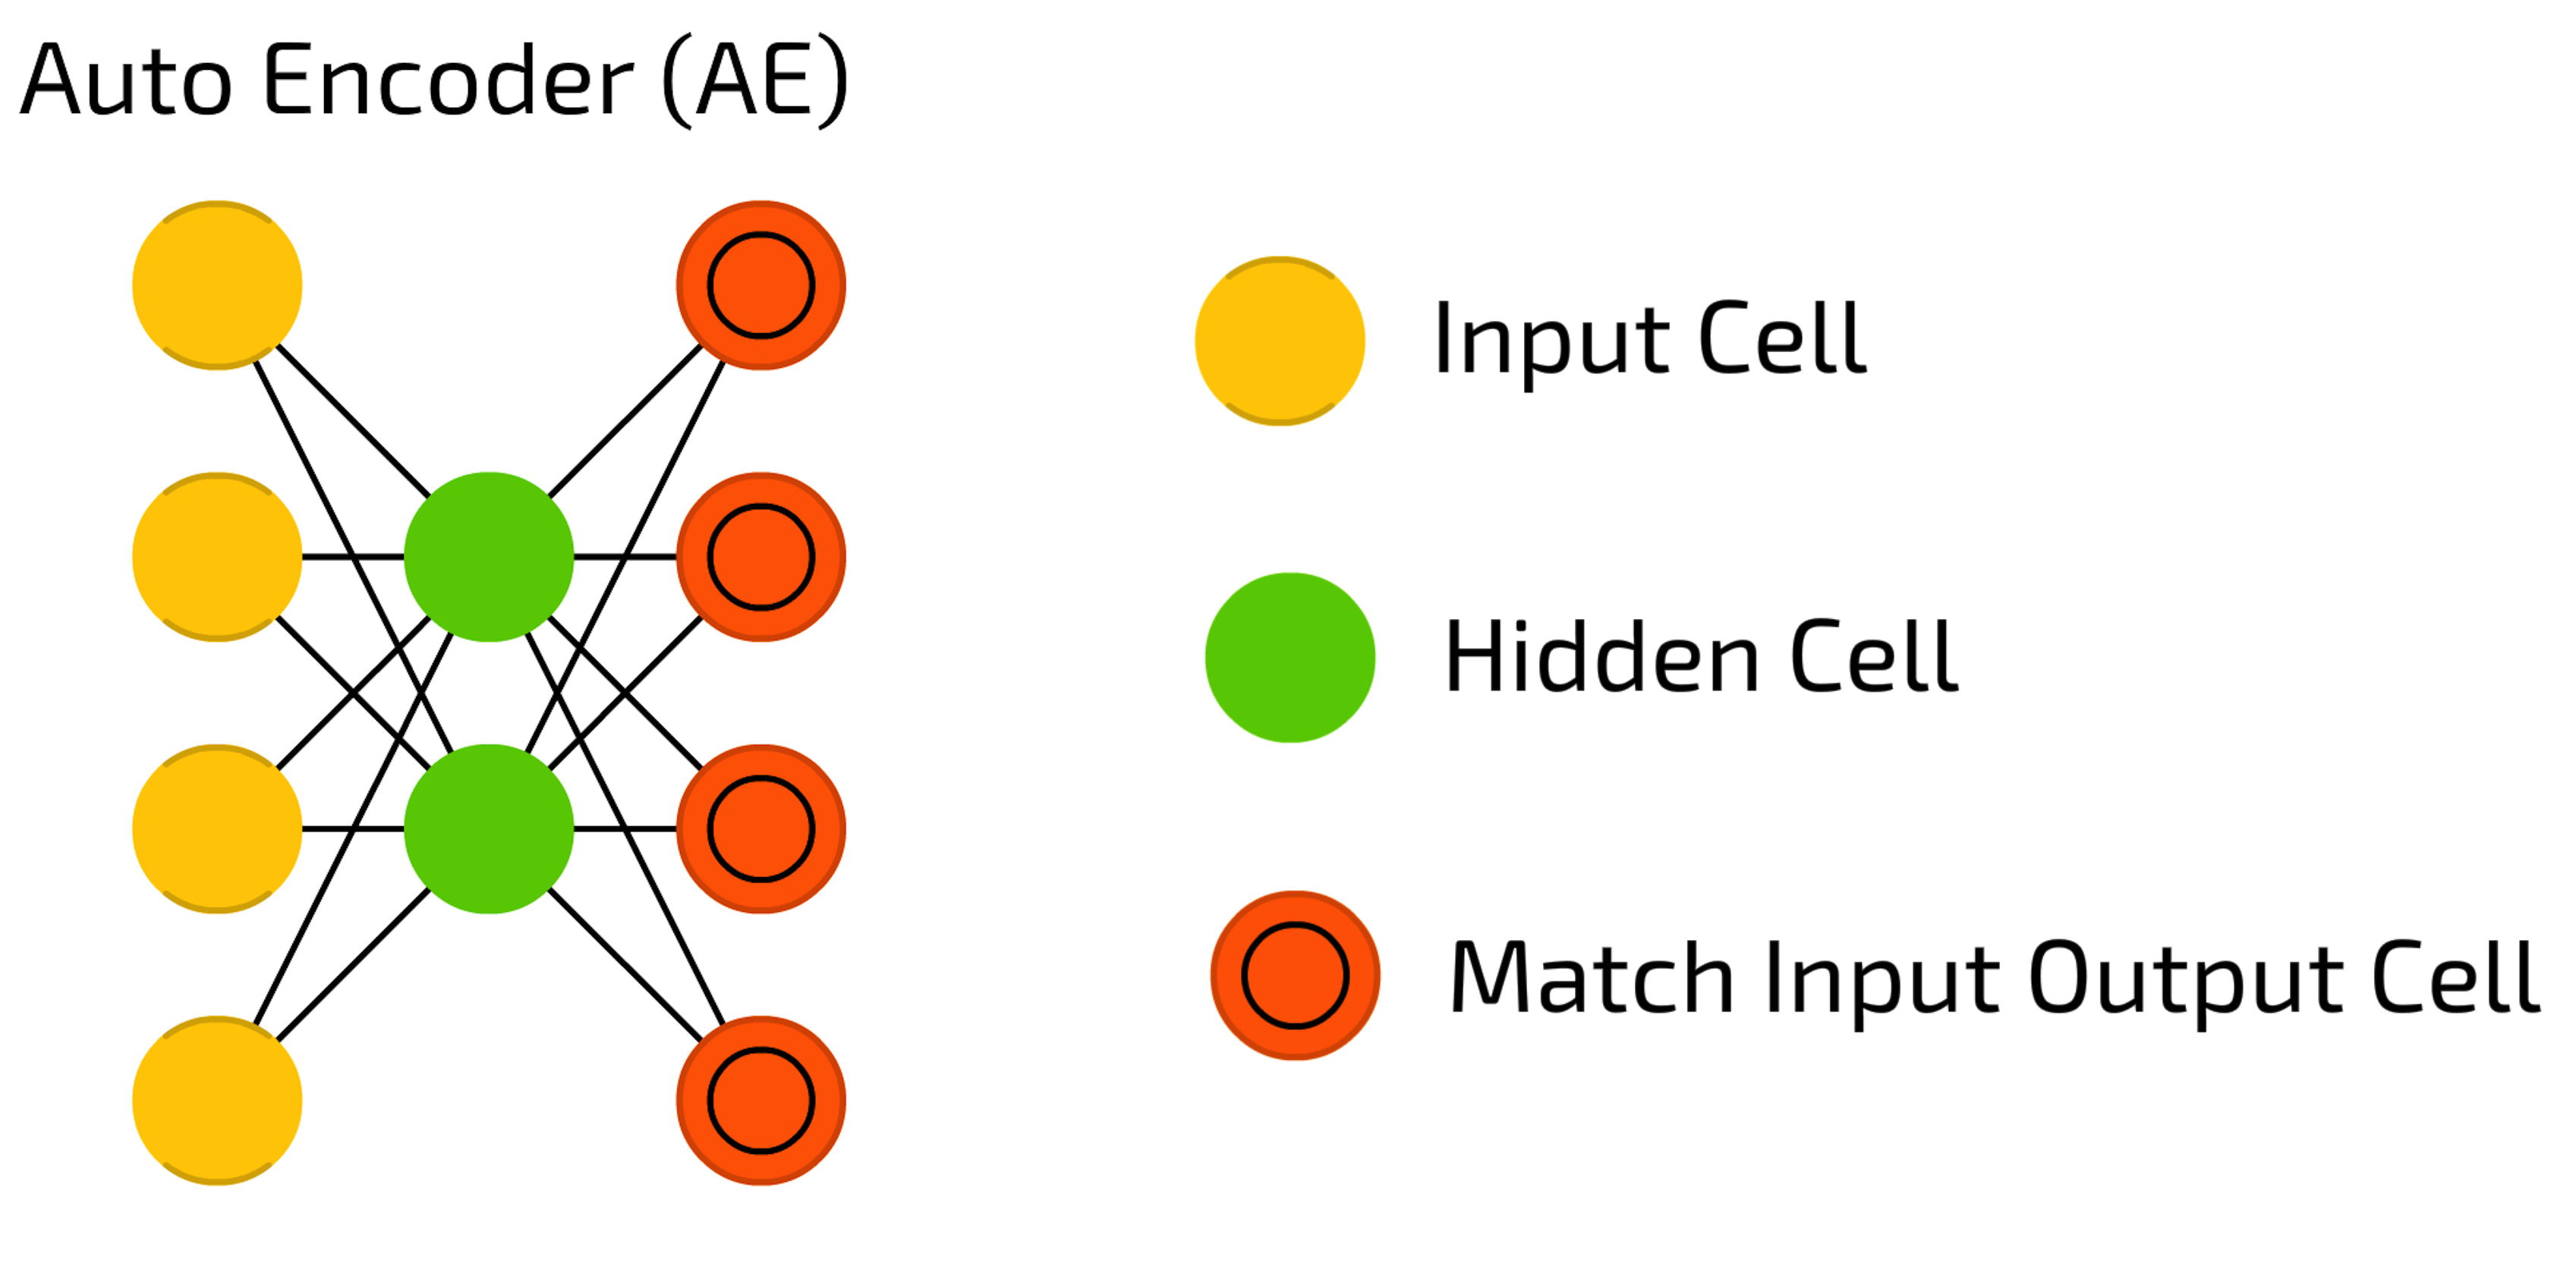
\includegraphics[width=0.9\textwidth]{pics/AE}
	\caption{Автокодировщик}
	\label{ae}
\end{figure}

Одно из основных предназначений автокодировщиков~--- снижение размерности исходного 
пространства. Сама процедура обучения нейросети заставляет автокодировщик запоминать 
основные признаки объектов, по которым будет проще восстановить исходные объекты выборки.
Чаще всего во время обучения в качестве функции потерь выбирают средний квадрат ошибки:
\[
	\mathsf{MSE}\bigl[g(f(X)), X\bigr] = \mathsf{MSE}(\hat{X}, X).
\]
Здесь возможно провести аналогию с методом главных компонент 
(англ. principal component analysis, PCA) \cite{pca}. 
Это метод снижения размерности, результатом работы которого является 
проекция выборки на подпространство, в котором дисперсия этой выборки максимальна.

По~сути автокодировщик является обобщением метода главных компонент: 
если ограничиться рассмотрением линейных моделей, автокодировщик 
и метод главных компонент дают одинаковые векторные представления \cite{autoenc_vs_pca}. 
Разница возникает, если в качестве энкодера и декодера выбраны
более сложные модели, например, многослойные \textit{полносвязные нейронные сети}.

\pagebreak
Как правило, размерность внутреннего представления меньше, чем размерность входного 
и выходного слоёв. Однако размерность латентного пространства не должна быть слишком маленькой,
иначе модель может потерять обобщающие способности. В~то~же время она не должна быть слишком
большой, чтобы не <<заучивать>> исходные данные (проблема переобучения \cite{overfeed}).


\section{Рекуррентная нейронная сеть}

Рекуррентная нейронная сеть (рекуррентная НС, англ. Recurrent neural network, RNN)~--- нейронная сеть, в которой разрешены циклы. 
Выход нейрона может подаваться снова на~вход этого~же нейрона,
на~вход всех нейронов в~текущем слое либо к~любому другому нейрону в~любом слое.

Рекуррентные НС хорошо подходят для работы с последовательностями данных именно по той причине, что
в них есть циклические соединения, через которые поступает информация с~предыдущих шагов
работы сети. Иными словами, рекуррентные НС могут анализировать входные данные не просто 
как набор изолированных друг от друга моментов времени, а как последовательность данных, 
где каждый последующий момент времени может некоторым образом зависеть или не зависеть от~предыдущих состояний:
\begin{figure}[!h]
	\centering
	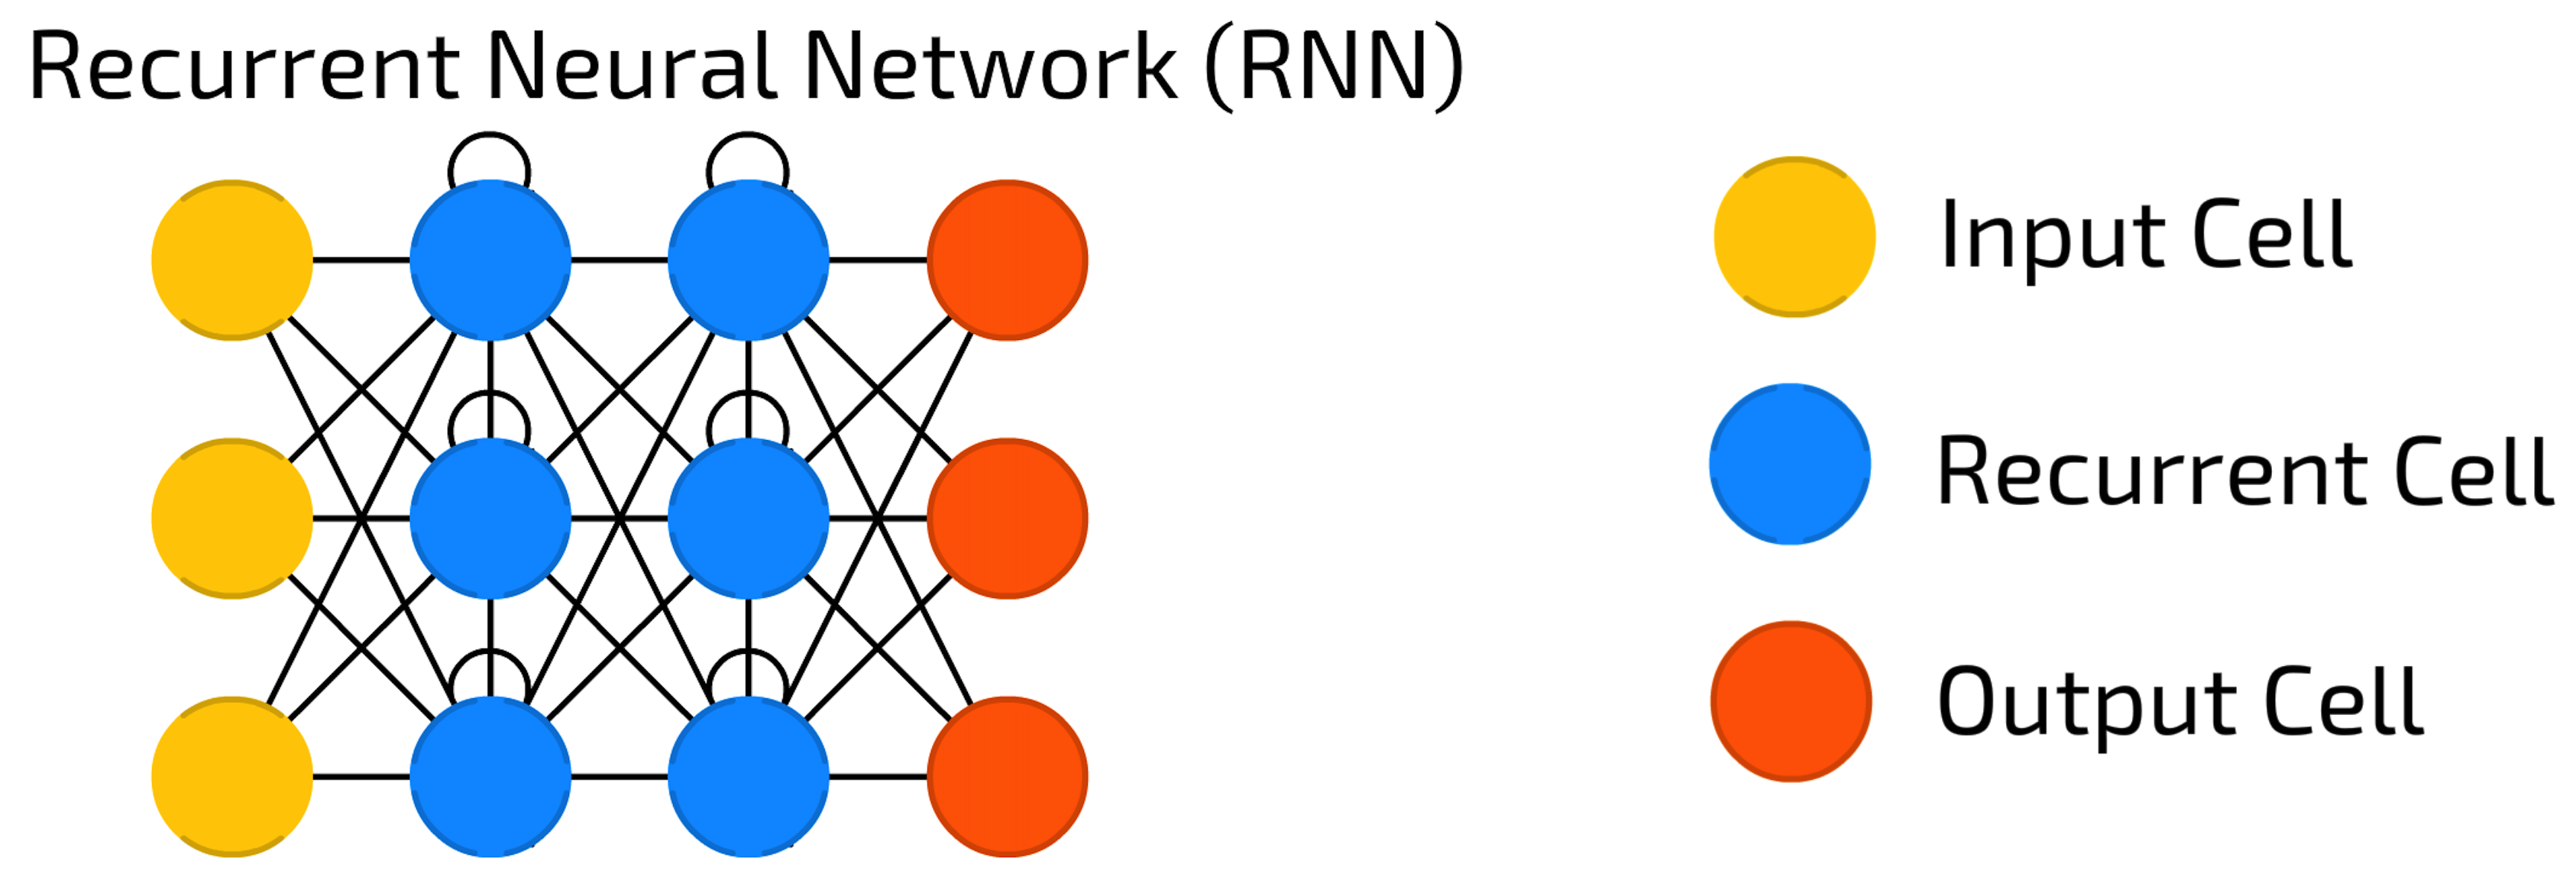
\includegraphics[width=0.75\textwidth]{pics/RNN}
	\caption{Рекуррентная НС}
	\label{RNN}
\end{figure}

\clearpage
Для обучения рекуррентной НС используется все тот же алгоритм обратного распространения ошибки. 
Рекуррентные НС представляют в виде НС с прямым распространением сигнала. Для этого используется 
\textit{разворачивание во времени} \cite{rnn_backprop}, при котором создается несколько копий рекуррентной НС. 
Выглядит это следующим образом:
\begin{figure}[!h]
	\centering
	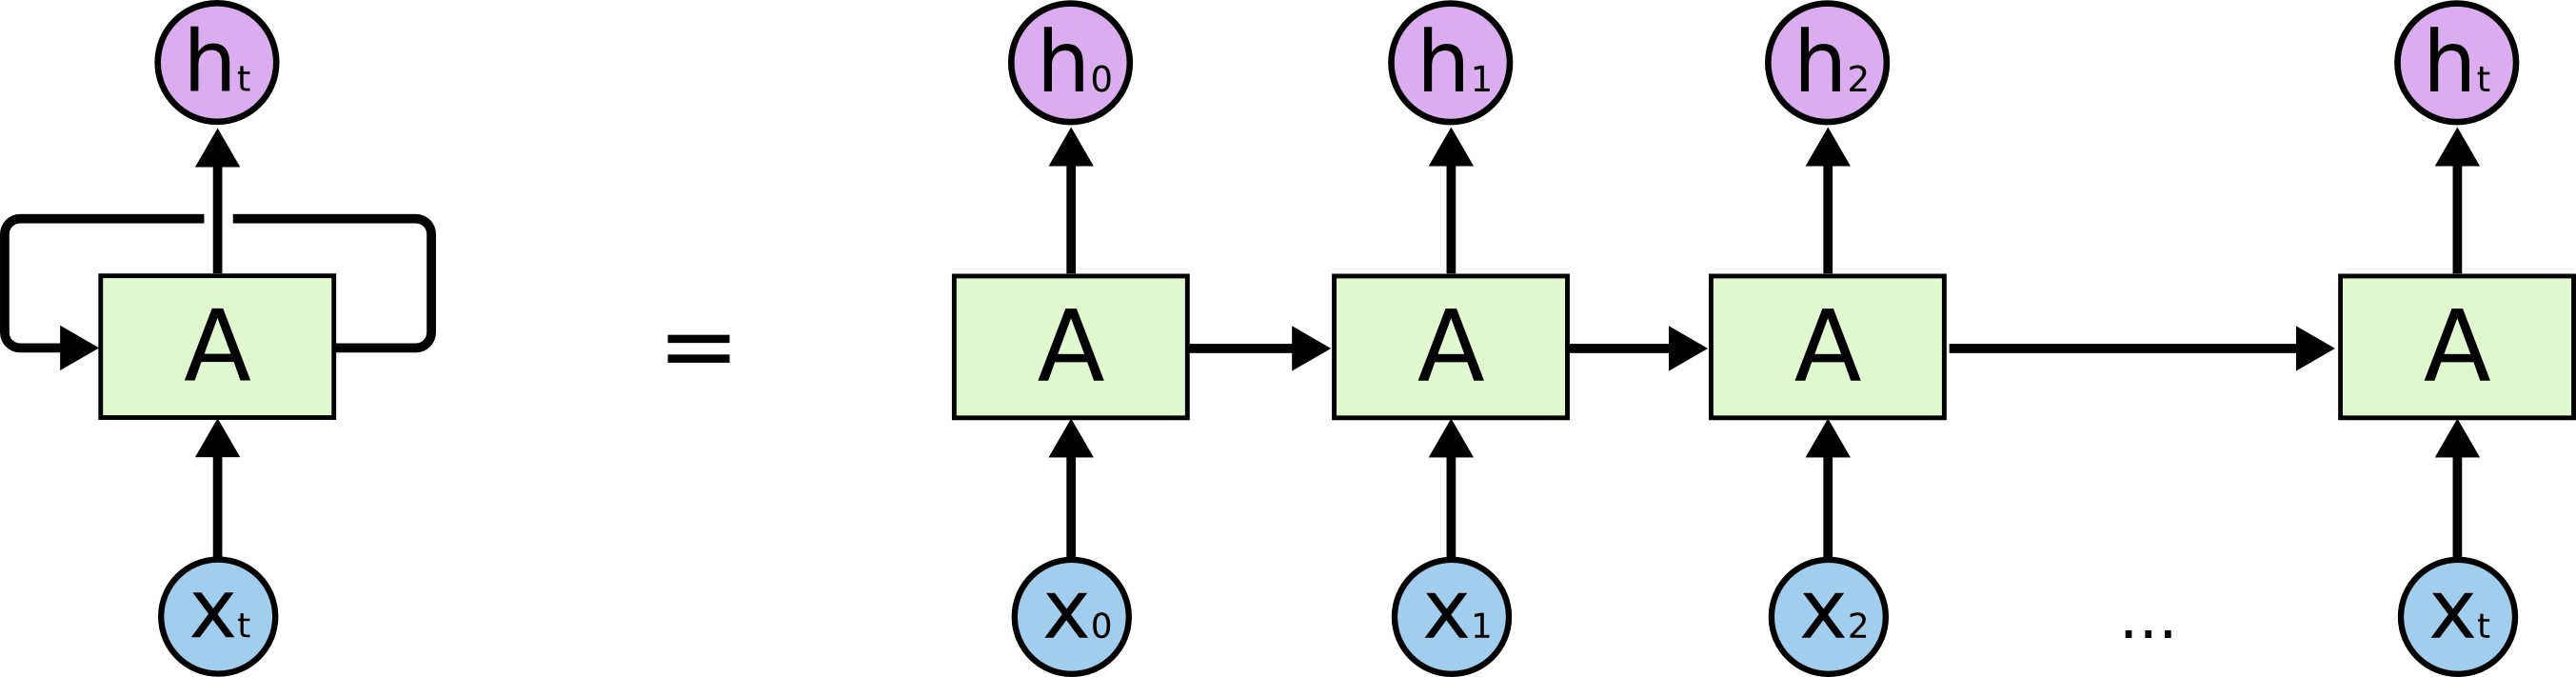
\includegraphics[width=0.9\textwidth]{pics/unpack}
	\caption{РНС и ее развернутое представление}
	\label{unpack}
\end{figure}
% нужно бы пояснить, что за h & x

Поскольку одни и те же параметры используются на всех временных этапах в сети, градиент на каждом выходе зависит не только от расчетов текущего шага, но и от предыдущих временных шагов.
%Например, чтобы вычислить градиент для четвертого элемента последовательности, нам нужно было бы «распространить ошибку» %на 3 шага и суммировать градиенты:
%\begin{figure}[!h]
%	\centering
%	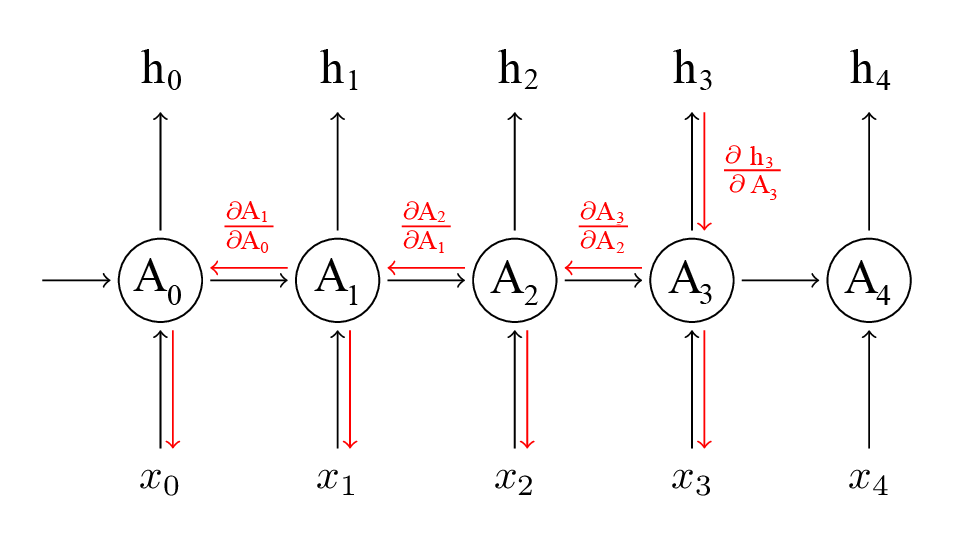
\includegraphics[width=0.8\textwidth]{pics/BPTT}
%	\caption{РНС и ее развернутое представление}
%	\label{BPTT}
%\end{figure}
Этот алгоритм называется \textit{алгоритмом обратного распространения ошибки сквозь время} 
(англ. Backpropagation Through Time, BPTT) \cite{BPTT}.

Рассмотрим некоторые реализации рекуррентных нейронных сетей, который используются в данной 
дипломной работе.

\subsection{Нейронная сеть Элмана}\label{elman}

Нейронная сеть Элмана~--- классический вариант рекурернтной нейронной сети. Она состоит из трех слоев: входного $ x $,
скрытого $ h $, и выходного $ z $ (см. рис.~\ref{simple_rnn}).
Для каждого элемента входной последовательности в~момент времени $ t $ 
вычисляется новое состояние по~следующему правилу:
\begin{align*}\label{h_t}
		&h_t = \tanh(W_{xh} x_t + b_{ih} + W_{hh} h_{(t-1)} + b_{hh}),\\
		&z_t = W_{hz}h_t + b_z,
\end{align*}
где $ h_t $~--- скрытое состояние в момент времени $ t $, $ x_t $~--- входные данные в момент 
времени $ t $, $ h_{t-1} $~--- скрытое состояние на предыдущем шаге в момент времени $ t {-} 1$ или 
начальное состояние в~момент времени 0, $ \tanh\left[ \circ \right] $~--- функция активации (гиперболический тангенс), схему слоя см. на~рис.~\ref{RNN_layer}

\begin{figure}[!h]
	\centering
	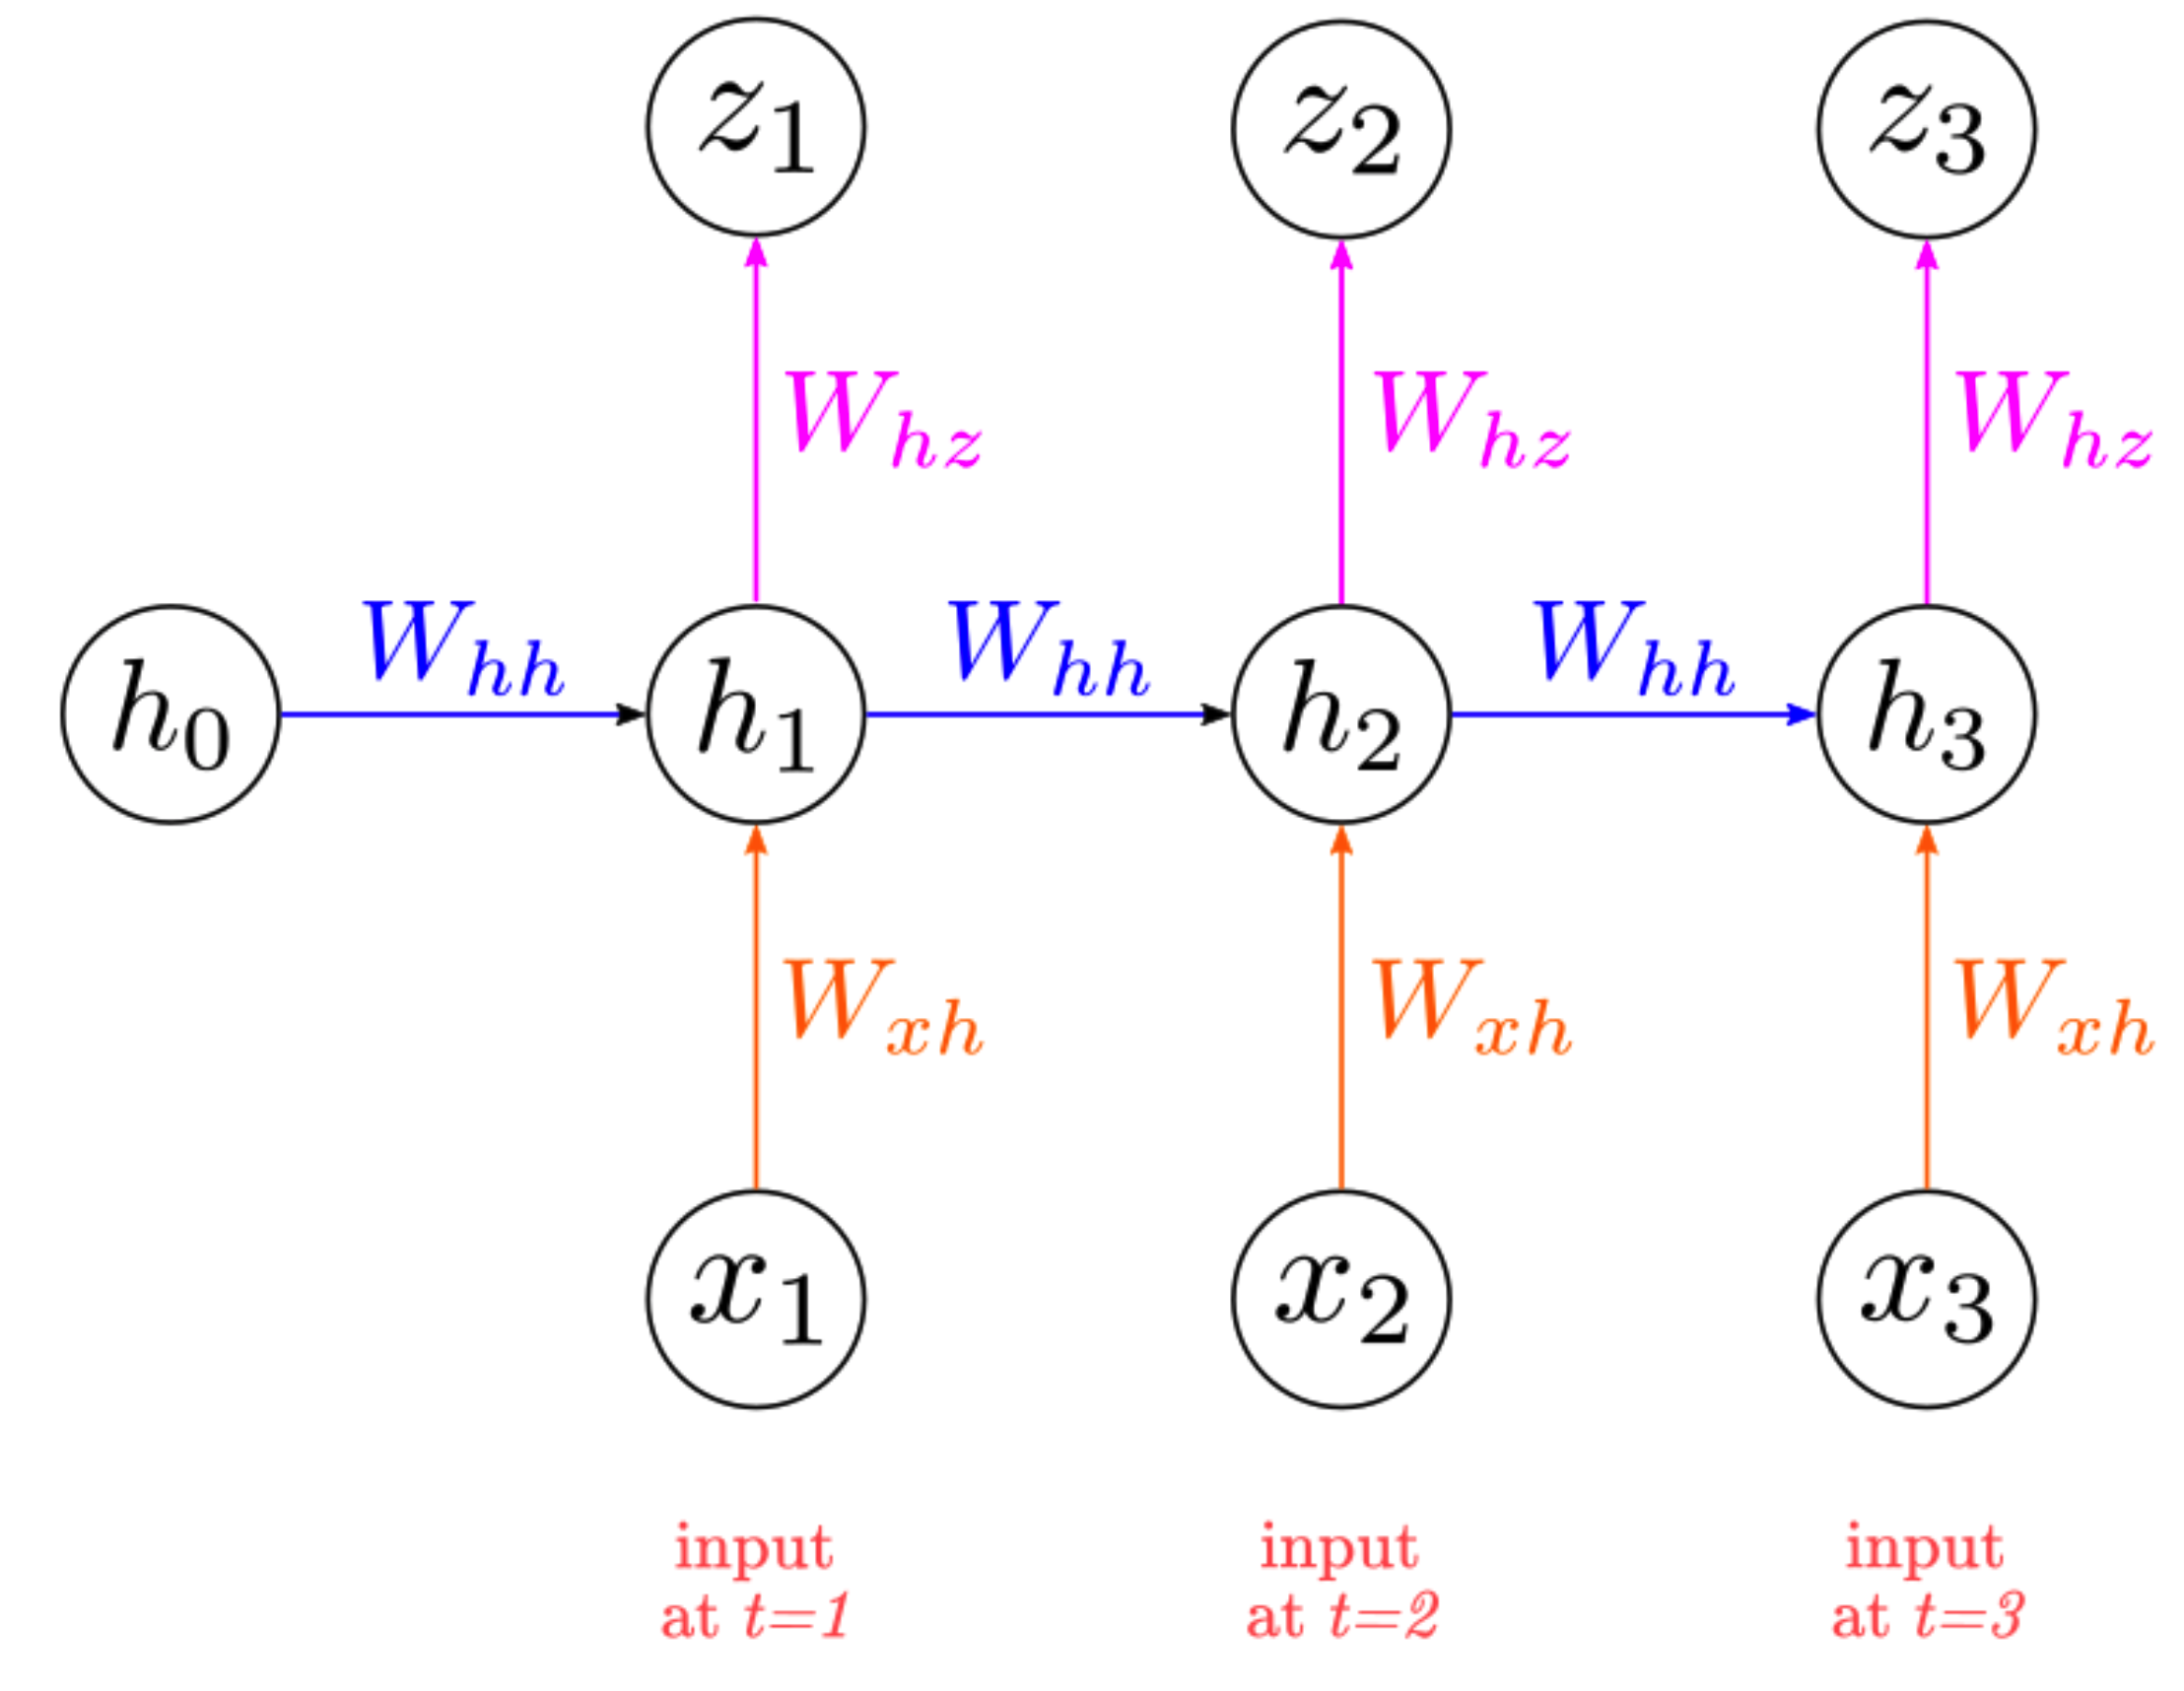
\includegraphics[width=0.5\textwidth]{pics/simple_rnn}
	\caption{Простейшая РНС}
	\label{simple_rnn}
\end{figure}

\begin{figure}[!h]
	\centering
	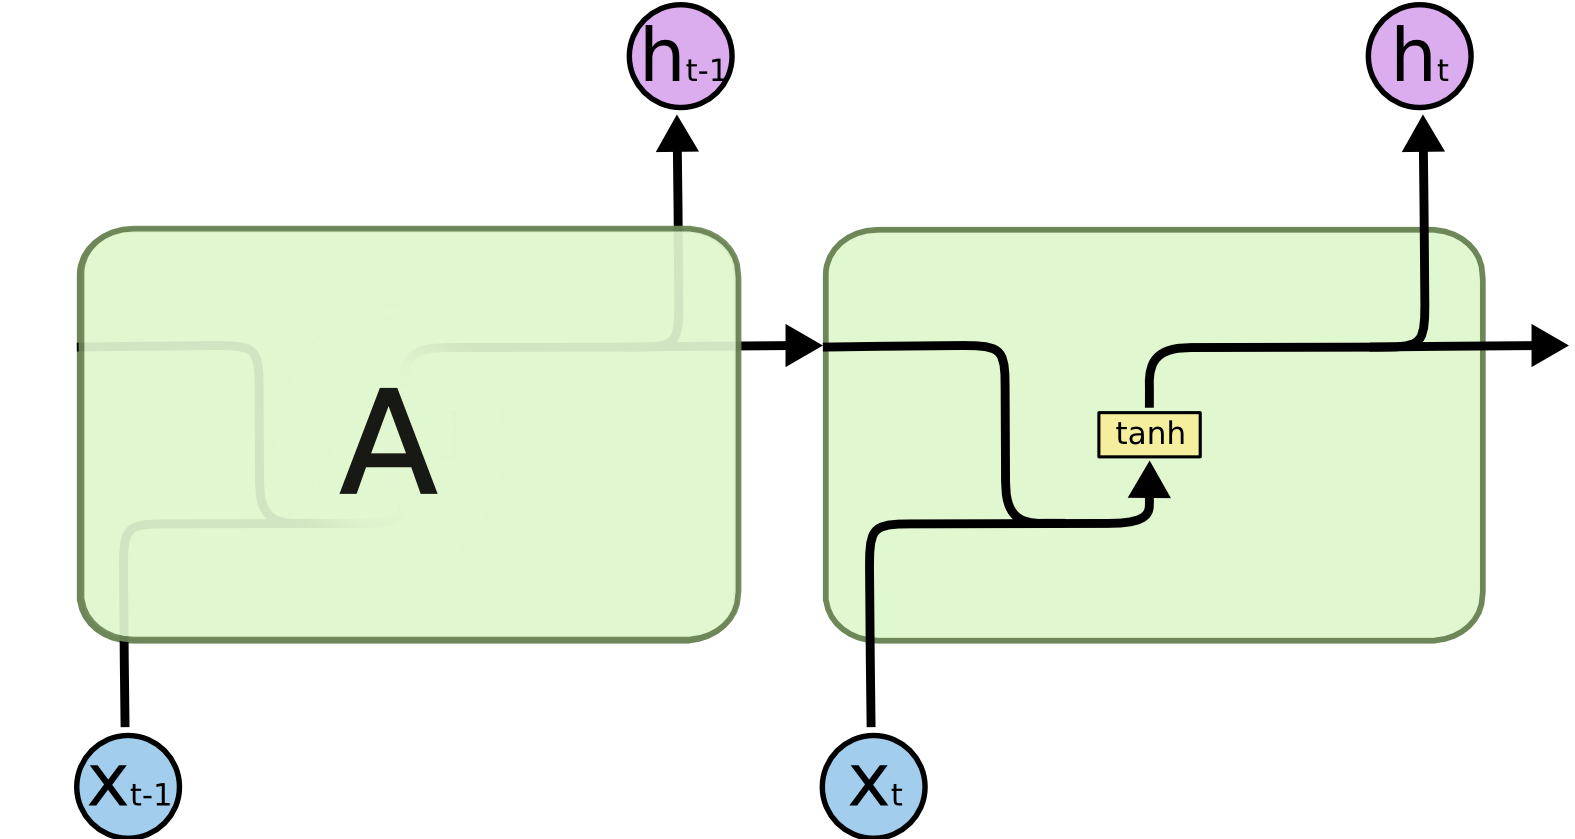
\includegraphics[width=0.8\textwidth]{pics/RNN_layer}
	\caption{Схема слоя рекуррентной сети}
	\label{RNN_layer}
\end{figure}

На каждом шаге на вход поступает информация, которая проходит прямой путь к выходному слою 
в~соответствии с~правилами обучения. Обратные связи сохраняют предыдущие значения 
скрытого слоя. Таким способом сеть сохраняет своё состояние, что может использоваться в предсказании 
последовательностей.

Однако если входная последовательность данных достаточно длинная (например, текст из~более чем сотни слов), то~такая простая сеть просто <<забудет>> слова, которые были в~начале. Поэтому при~необходимости
проводить анализ длинных последовательностей необходимо научить нейронную сеть хорошо запоминать
важные паттерны.

Другая проблема длинных последовательностей данных~--- большое количество слоев НС. Из-за этого
снова встает вопрос о быстром затухании градиентов ошибок. 
Чтобы решить эти проблемы, были придуманы специальные блоки, заменяющие <<обычные>> нейроны.

\subsection{Управляемые рекуррентные блоки}\label{GRU}

Управляемые рекуррентные блоки (англ. Gated Recurrent Units, GRU)~--- механизм вентилей для рекуррентных нейронных сетей.
Для каждого элемента входной последовательности в~момент времени $ t $ 
вычисляется новое состояние по~следующему правилу:
\begin{align*}
	&r_t = \sigma(W_{xr} x_t + b_{ir} + W_{hr} h_{(t-1)} + b_{hr}); \\
	&z_t = \sigma(W_{xz} x_t + b_{iz} + W_{hz} h_{(t-1)} + b_{hz}); \\
	&n_t = \tanh\left[ (W_{xn} x_t + b_{in}) + r_t \cdot (W_{hn} h_{(t-1)}+ b_{hn})\right]\!{;} \\
	&h_t = (1 - z_t) \cdot n_t + z_t \cdot h_{(t-1)},
\end{align*}
где $ h_t $~--- скрытое состояние в момент времени $ t $, $ x_t $~--- входные данные в момент 
времени $ t $, $ h_{t-1} $~--- скрытое состояние на предыдущем шаге в~момент времени $ t {-} 1$ или 
начальное состояние в~момент времени 0, $ r_t $, $ z_t $, $ n_t $~--- вентиль сброса, вентиль обновления и 
новый вентель соответственно, $ \tanh \left[ \circ \right] $~--- функция активации (гиперболический тангенс).  

\clearpage
Основная идея таких блоков заключается в том, что обычный нейрон заменяется 
на некоторый блок, у которого есть память и есть вентили, которые контролируют сброс, перезапись или сохранение этой памяти.
Данный блок схематично можно изобразить следующим образом:
\begin{figure}[!h]
	\centering
	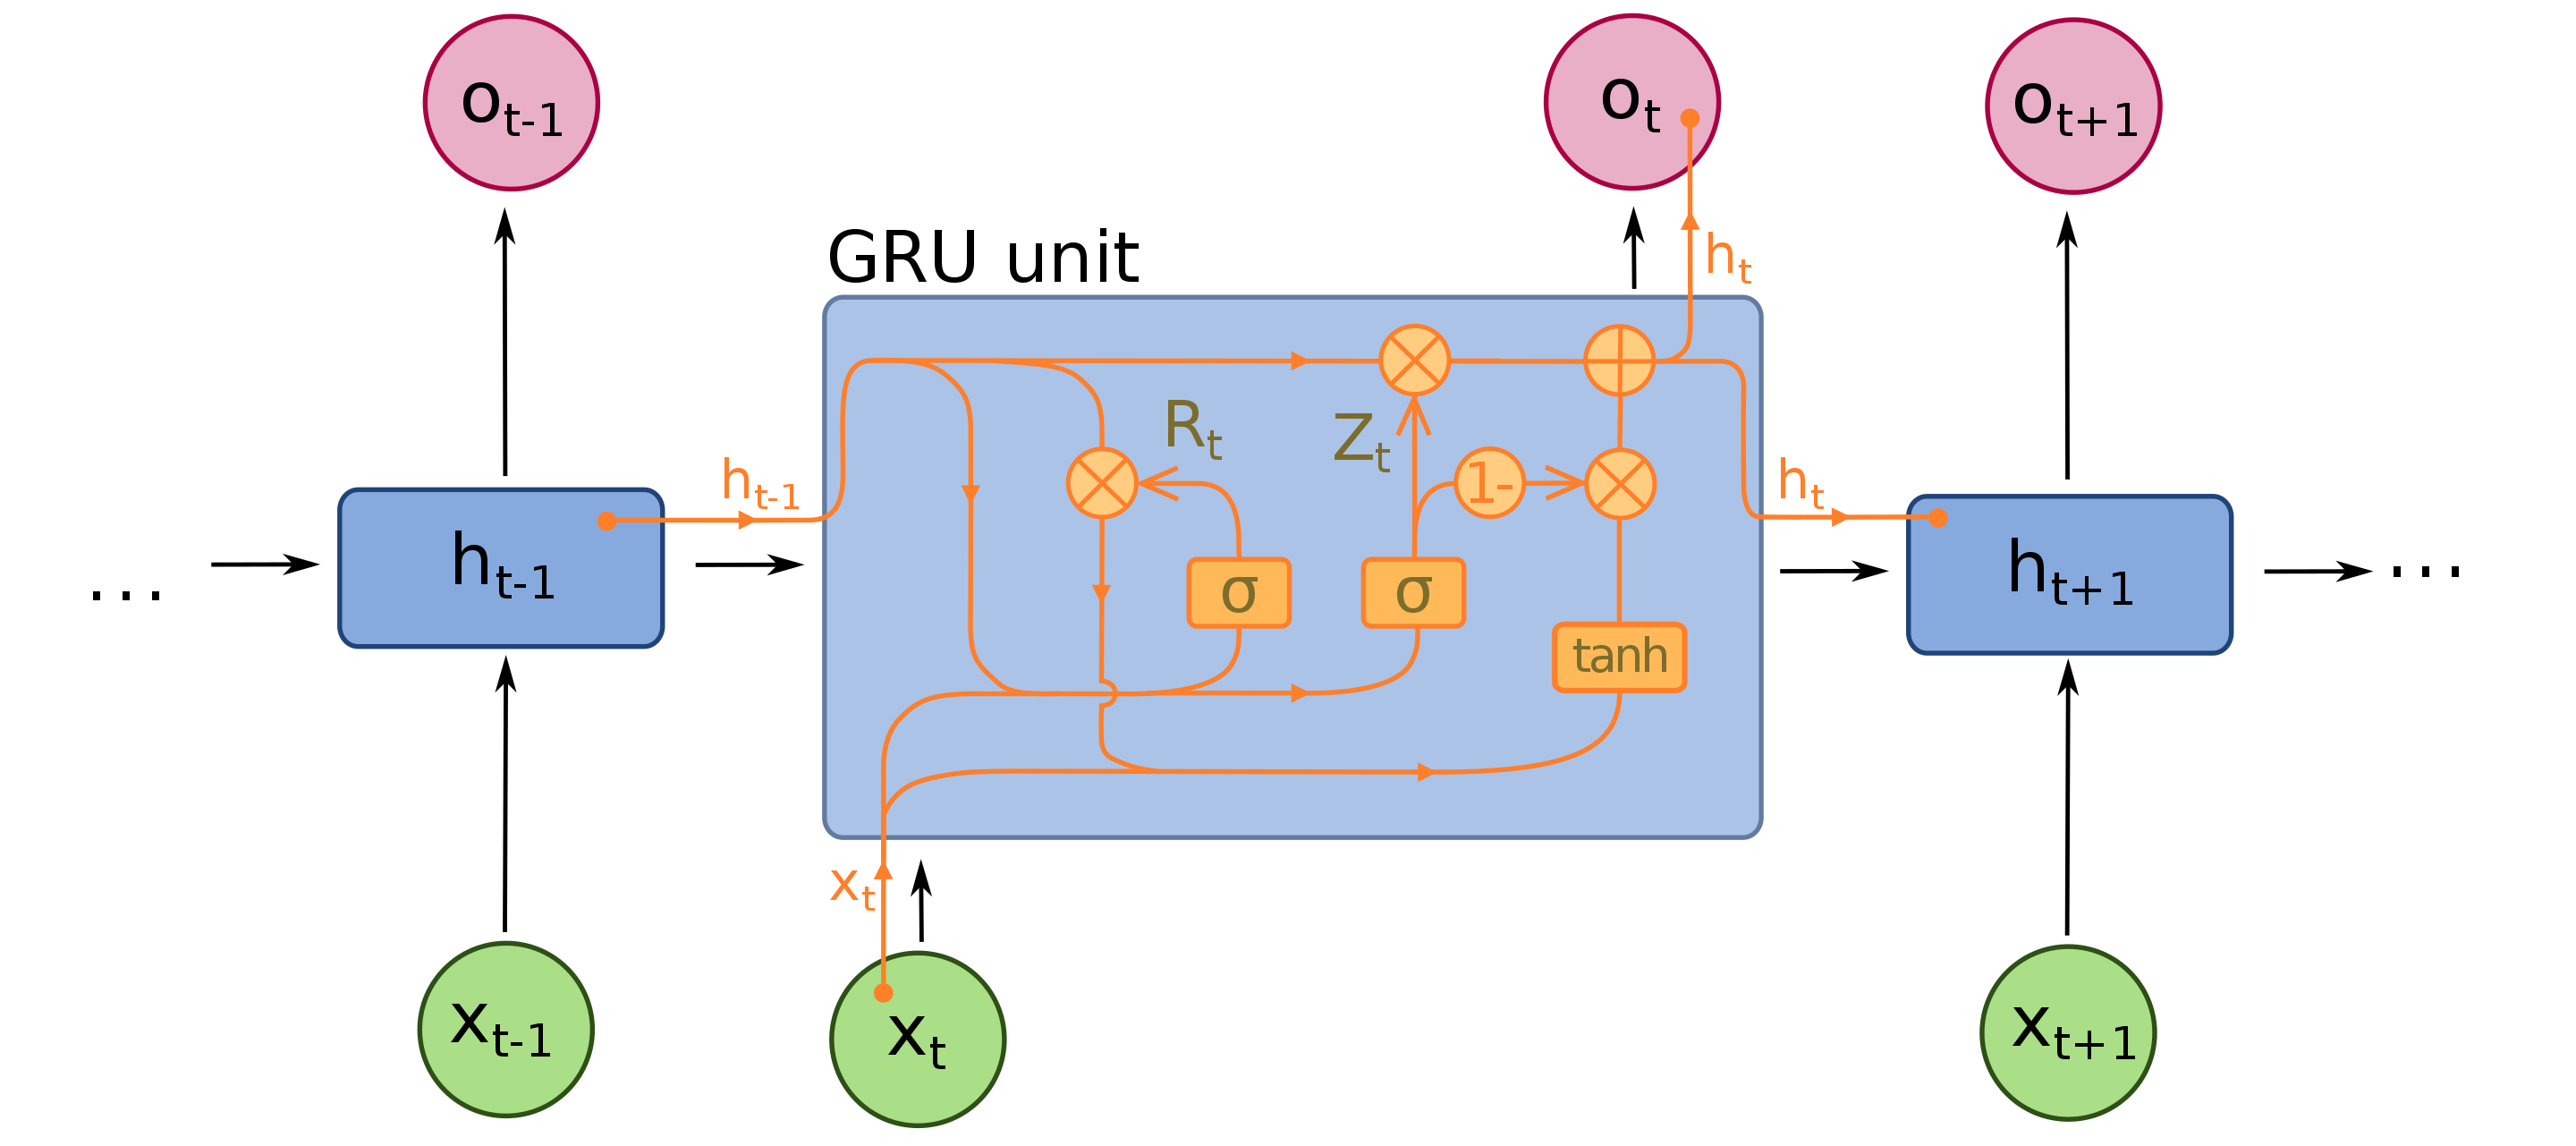
\includegraphics[width=0.9\textwidth]{pics/gru_layer}
	\caption{Схема слоя с управляемым рекуррентным блоком}
	\label{gru_layer}
\end{figure}

Нейронные сети, в которых используется данный подход, как правило, превосходят \cite{rnn_compare}
классические рекуррентные сети.
